\section{Euler Angles}
One method of describing coordinate system transformations, are the Euler angles.
They serve as a mathematical tool to connect one CS with another.\\
The initial coordinate system $\textbf{x},\textbf{y},\textbf{z}$,
shown in Fig. \ref{fig:EulerAngles} can be transformed into the $\textbf{x}',\textbf{y}',\textbf{z}'$ CS by three rotations.
The three Euler angles $\alpha$, $\beta$ and $\gamma$ are defined as follows.
The distance between the vectors $\textbf{L}_\mathrm{a}$ and $\textbf{L}_\mathrm{b}$ is shown in red.
This is the cutting line $\textbf{L}$ between the $\textbf{xy}$ and $\textbf{x'y'}$ planes.
Here, $\alpha$ is the angle between $\textbf{x}$ and $\textbf{L}_\mathrm{a}$ and $\beta$ is the angle between the two z--axes $\textbf{z}$ and $\textbf{z}'$.
The angle $\gamma$ is the angle between $\textbf{L}_\mathrm{a}$ and $\textbf{x}'$. 
The transformation of the CS requires three rotations in a specific order.\\

\begin{figure}[H]
    \centering
	\vspace*{-1.3cm}
    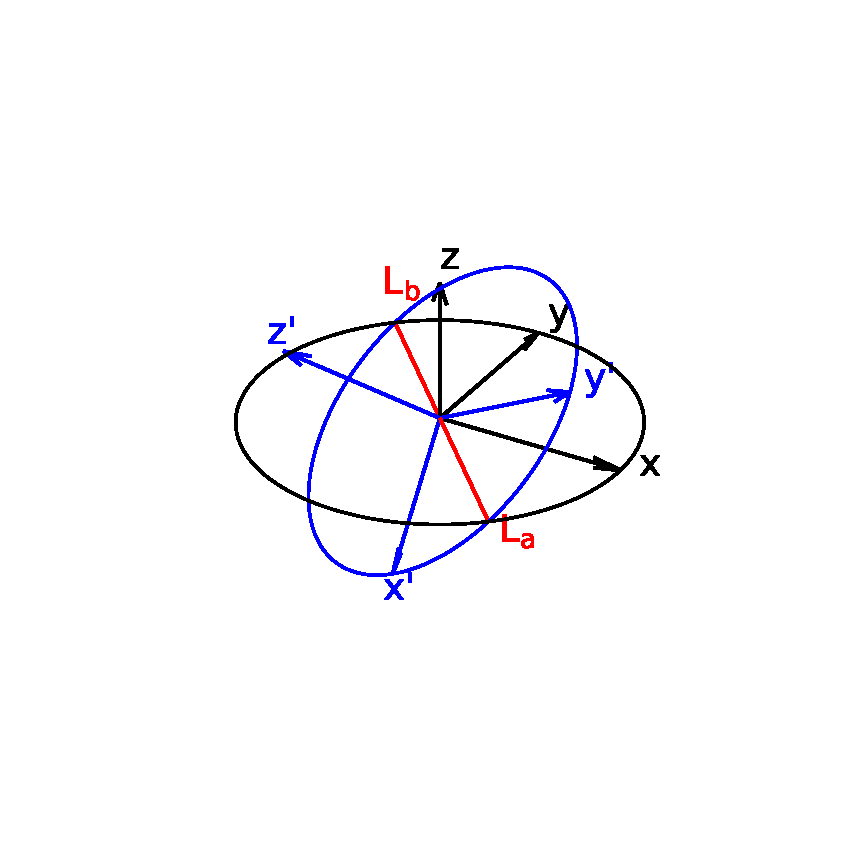
\includegraphics[width = 0.8\textwidth]{sections/TheoryGraphs/EulerAngle.eps}
	\vspace*{-2cm}
    \caption[Depiction of two Coordinate systems for description of Euler Angles.]{ Depiction of two coordinate systems  $\textbf{x},\textbf{y},\textbf{z}$ (black) and $\textbf{x}',\textbf{y}',\textbf{z}'$ (blue). 
			   The red cutting line of the $\textbf{xy}$ and $\textbf{x'y'}$ planes is between the vector $\textbf{L}_\mathrm{a}$ and $\textbf{L}_\mathrm{b}$.}
    \label{fig:EulerAngles}
\end{figure}

For the rotation of the CS it is necessary to apply the rotation matrices in a specific order.
The first rotation is around $\textbf{z}$ by the angle $\gamma$, followed by the rotation $\textbf{x}$ by $\beta$.
Then a rotation around the $\textbf{z}$ axis is done by the angle $\alpha$.
The rotation matrices $\textbf{R}_z(\theta)$, and $\textbf{R}_x(\theta)$ are mathematically described 
in Eq.~\eqref{eq:rotMatZ} and Eq.~\eqref{eq:rotMatX}, respectively.
These are the rotation matrices for a classical rotation around the $\textbf{z}$ and $\textbf{c}$ axes.
\begin{align}
	\label{eq:rotMatZ}
	\textbf{R}_z (\theta)  = \left(\begin{matrix}
					\cos(\theta) & -\sin(\theta) & 0 \\
					\sin(\theta) & \cos(\theta) & 0 \\
					0 & 0 & 1 \\
					\end{matrix} \right)
\end{align}

\begin{align}
	\label{eq:rotMatX}
	\textbf{R}_x (\theta)  = \left(\begin{matrix}
						1 & 0 & 0 \\
						0 & \cos(\theta) & -\sin(\theta)  \\
						0 & \sin(\theta) & \cos(\theta) \\
					\end{matrix} \right)
\end{align}

The full rotation of the coordinate system in dependency of the Euler angles is shown in Eq.~\eqref{eq:R_Euler}.

\begin{align}
	\label{eq:R_Euler}
	\textbf{R} = \textbf{R}_z (\gamma) \times \textbf{R}_x (\beta) \times \textbf{R}_z (\alpha)
\end{align}

\section{Electronic Structure Theory}
	In this report, properties derived from electronic structure theory are used for the training of the ML models.
	Although GFN2--xTB is used for this purpose, a short introduction to the Hartree--Fock model and Density Functional Theory is given.
	The introduction starts from the non--relativistic, stationary electronic Schrödinger--equation.
	From this the Hartree--Fock model will be derived.
	This is followed by Density Functional Theory, as this builds the theoretical basis of GFN2--xTB.
	After that the tight--binding method will be introduced from which the semiempirical method GFN2--xTB is derived.
	Atomic units are used for all equations in this section.

	\subsection{Hartree--Fock Model}
	Molecular systems in quantum mechanics can be described by a many--body wave function eigenvalue problem.
	The solution of this problem is given by solving the Schrödinger equation. The separation of its time--dependency, neglecting relativistic effects and
	the introduction of the \mbox{Born--Oppenheimer (BO) approximation} results in the electronic Schrödinger equation (Eq.~\eqref{eq:eSGl}).
	\begin{align}
		\label{eq:eSGl}
		\hat{H}_\mathrm{e} \Psi_\mathrm{e} = E_\mathrm{e} \Psi_\mathrm{e}
	\end{align}
 	The solution of this eigenvalue equation leads to the electronic energy $E_\mathrm{e}$.
	The electronic many--body--wave function $\Psi_\mathrm{e}$ of the system can be described by the Slater determinant (Eq.~\eqref{eq:SlaterD}).
	The use of the Slater determinant fulfills the condition of the antisymmetry of the wave function.
	The condition is due to the Pauli exclusion principle.
	The Slater determinant consists of $k$ spin--orbital wave functions $\phi_i$,
	and every wave function is permuted with the coordinates $\textbf{r}_i$ of the $N$ electrons.
	Furthermore, the wave function is normalized by the factor $(N!)^{-\frac{1}{2}}$.
	\begin{align}
		\label{eq:SlaterD}
		\Psi_\mathrm{e} = \dfrac{1}{\sqrt{N!}} \begin{vmatrix}
			\phi_1(\textbf{r}_1) & \phi_2(\textbf{r}_1)& \hdotsfor{1}&  \phi_k(\textbf{r}_1)\\
			\phi_1(\textbf{r}_2) &  \phi_2(\textbf{r}_2) & & \vdots\\
			\vdots& & \ddots& \vdots \\
			\phi_1(\textbf{r}_N)& \hdotsfor{1}& \hdotsfor{1} & \phi_k(\textbf{r}_N)\\
		\end{vmatrix}
	\end{align}
	The electronic Hamiltonian $\hat{H}_\mathrm{e}$ in the Hartree--Fock model is shown in Eq.~\eqref{eq:effHamiltonian}
	and consists of the kinetic energy of the electrons and the potential energy between electrons and nuclei as also between the electrons.
	Furthermore, the nuclear repulsion energy, which is approximated as a constant, is added.
	The kinetic energy of the nuclei can is separated, due to the \mbox{BO--approximation}.
	% Instead of the computation of every electron--electron interaction,
	% the electrons are assumed to be in an effective electronic potential,
	% which simplifies the hamiltonian to a sum of effective one--electron hamiltonians.
	% This is depicted in Eq.~\eqref{eq:effHamiltonian}.
	\begin{align}
		\label{eq:effHamiltonian}
		\hat{H}_\mathrm{e} = \sum_{A = 1}^{M} \sum_{i=1}^N \left( -\dfrac{1}{2}\nabla_i^2 - \dfrac{1}{|\textbf{R}_A - \textbf{r}_i|}\right) 
		+ \sum_{i=1}^N \sum_{\substack{j = 1 \\ i>j}}^N \dfrac{1}{|\textbf{r}_{i} - \textbf{r}_{j}|} 
		+ \sum_{A=1}^M \sum_{\substack{B=1\\ B>A}}^M \dfrac{Z_A Z_B}{|\textbf{R}_A - \textbf{R}_B|}
	\end{align}
	Here, $\textbf{R}_A$ is the coordinates of atom $A$, 
	$\textbf{r}_i$ the coordinates of electron $i$ and $Z_A$ the nuclear charge.
	While, $\nabla_i^2$ is the second derivative in respect to every coordinate of electron $i$.\\
	The electronic energy can now be described with the Slater determinant and Hamiltonian in Eq.~\eqref{eq:ElectronicEnergy}
	This leads to the description of the energy by the one--electron operator $h_i$,
	the coulomb operator $\hat{J}_i$ and the exchange operator $\hat{K}$.
	\begin{align}
		\label{eq:ElectronicEnergy}
		E_\mathrm{e} = \sum_{i=1}^N \braket{\phi_i | h_i | \phi_i} 
		+ \dfrac{1}{2} \sum_{i=1}^N \sum_{j=1}^N \left(\braket{\phi_j | \hat{J}_i | \phi_j} 
		- \braket{\phi_j | \hat{K}_i | \phi_j}\right)
	\end{align}

	The Rayleigh--Ritz variational principle (s. Eq.~\eqref{eq:RayleighRitzVP}) states,
	that the total energy $E_0$ of the system is always beneath or equal
	to the energy corresponding to the approximated wave function.
	This allows the search of the exact energy by optimizing the wave function (or its parameters).
	\begin{align}
		\label{eq:RayleighRitzVP}
		E_0 \leq \braket{\Psi | \hat{H} | \Psi}
	\end{align}
	Hence, the determination of the total energy of the system is an eigenvalue problem and can be solved by minimization.
	To minimize the energy, Lagrangian optimization is employed, under the condition of orthonormal $\phi_i$.
	The inner product of the wave function $\braket{\phi_i|\phi_j} = \delta_{ij}$ corresponds to the Kronecker delta. 
	The Kronecker delta is $\delta_{ij} = 0$ if $i$ and $j$ are not equal, and $\delta_{ij} = 1$ if $i$ and $j$ are equal.
	The derivative of the Lagrangian functional leads to the canonical Fock equation \eqref{eq:FockEquation},
	which is a solution for the minimal energy.

	\begin{align}
		\hat{f}(\textbf{r}_i) \phi_k(\textbf{r}_i) &= \epsilon(\textbf{r}_i) \phi_k(\textbf{r}_i)
		\label{eq:FockEquation}\\
		\hat{f}(\textbf{r}_i) &= \hat{h} + \sum_{j=1}^N (2 \hat{J}_j - \hat{K}_j)
	\end{align}

	The Fock--operator $\hat{f}(\textbf{r}_i)$ is an effective one--electron operator.
	This enables the determination of the spin--orbital wave functions in an iterative manner,
	as the Fock--operator itself depends on the spin--orbital wave functions.
	The iterative search is possible due to the self--consistency of the Hartree--Fock equation.
	Furthermore, the general optimization can be achieved due to the Rayleigh--Ritz variational principle.
	Important to point out is that the Fock--operator consists of the one--electron operator, the exchange--operator
	and the coulomb operator, while the correlation is not included. \\
	The spin--orbital wave functions are described via a basis set approximation.
	This LCAO--approach is shown in Eq.~\eqref{eq:BasisSet},
	where the spin--orbital wave--functions are the sum of $K$ basis functions with an associated constant.
	\begin{align}
		\label{eq:BasisSet}
		\phi_i(\textbf{r}) = \sum_\mu^K c_\mu \chi_\mu (\textbf{r})
	\end{align}
	Merging the basis--set approach into Eq.~\eqref{eq:FockEquation} leads to Roothaan--Hall equation shown in Eq.~\eqref{eq:FCSCe}.
	Here, $\textbf{F}$ is the Fock matrix, $\textbf{C}$ a matrix of coefficients $c_\mu$,
	$\textbf{S}$ the overlap matrix and $\bm{\upepsilon}$ the diagonal eigenvalue matrix.
	This equation is used find a solution for the energy iteratively.
	Starting with an initial guess of the Fock matrix,
	the matrix $\textbf{C}$ is computed, with this matrix, the density matrix $\textbf{D}$ is calculated. 
	From the matrix $\textbf{D}$, is then used for the calculation of the new Fock matrix.
	\begin{align}
		\label{eq:FCSCe}
		\textbf{F} \textbf{C} = \textbf{S} \textbf{C} \bm{\upepsilon}
	\end{align}
	% \textcolor{blue}{There is an infinite large number of possible solutions for the spin--orbital wave functions,
	% which leads to high computational cost and capacity for solving.
	% For the simplification, a basis set of a LCAO--approach is used for the computation of the spin--orbital wave function.}
	% \begin{align}
	% 	\phi(\textbf{r}) = \sum_\mu^K c_\mu \chi_\mu(\textbf{r})
	% \end{align}
	% \subsection{Kohn--Sham Density Functional Theory}
	% The molecule--orbital wave functions $\psi_i$ is approximated with basis sets, shown in Eq.~\eqref{eq:BasisSet}
	% \begin{align}
	% 	\label{eq:BasisSet}
	% 	\psi_i = \sum^{A}_{i} \chi 
	% \end{align}
	\subsection{Kohn--Sham Density Functional Theory}
	As mentioned above, the correlation between electrons is not described in the Hartree--Fock model,
	due to the use of a single Slater determinant.\\
	The correlation energy can be described by two different approaches.
	Instead of using one single Slater determinant, a linear combination of Slater determinants can be used.
	This leads to the post--Hartree--Fock methods like Full--CI or MP2.
	The second approach is the Density Functional Theory (DFT).\\
	The Hohenberg--Kohn theorems build the basis for the DFT.
	These two theorems postulate, that the energy is a functional of the density,
	and that this functional follows the variational principle.\\
	The description of the energy can therefore be done via the density of the electrons,
	which is defined in Eq.~\eqref{eq:Density}.
	Where, $n_\mathrm{occ}$ is the occupation number of the spin--orbital wave function.
	\begin{align}
		\label{eq:Density}
		\rho(\textbf{r}) = n_\mathrm{occ} \sum_{i=1}^n  |\phi_i(\textbf{r})|^2
	\end{align}
	The general approach is to describe the energy in dependence of the electron density $E[\rho]$.
	There are different approaches for this connection. 
	The most known approach, Kohn--Sham Density Functional Theory (KS--DFT), will be discussed.
	The energy in KS--DFT consists of the inexact kinetic energy, coulomb integral,
	the exchange correlation energy and the potential field.
	The kinetic energy is inexact, due to the assumption of non--interacting electrons.
	The energy $E_\mathrm{XC}$ consists mainly of the correlation energy and the exchange energy.
	In theory, the energy $E_\mathrm{XC}$ should also include the self interaction energy and a correction to the kinetic energy.
	\begin{align}
		\label{eq:EnergyDFT}
		E[\{\phi_i\}] = T[\{\phi_i\}] + J[\rho] + E_\mathrm{XC}[\rho] + \int v(\textbf{r}) \rho(\textbf{r}) \mathrm{d}\textbf{r}
	\end{align}
	The minimization of the energy is done by a Lagrangian optimization with analogue conditions compared to Hartree--Fock.
	This leads to the Kohn--Sham operator and a new eigenequation, which is shown in Eq~\eqref{eq:KSEigeneq}.
	\begin{align}
		\hat{f}^\mathrm{KS}(\textbf{r}_i) \phi_k(\textbf{r}_i) &= \epsilon(\textbf{r}_i) \phi_k(\textbf{r}_i)\label{eq:KSEigeneq}\\
		\hat{f}^\mathrm{KS}(\textbf{r}_i) &= \hat{h}_i + 2 \sum^n_{j=1} \hat{J}_j + \hat{v}_\mathrm{xc} 
	\end{align}
	In comparison to the Fock operator, $\hat{f}^\mathrm{KS}(\textbf{r}_i)$ includes an exchange--correlation term, instead of the exchange operator.
	With a basis set approach analogue to the HF model,
	an eigenvalue equation similar to the Roothaan--Hall equation is derived.
	% The spin--orbital wave functions are described via a basis set approximation.
	% This LCAO--approach is shown in Eq.~\eqref{eq:BasisSet},
	% where the spin--orbital wave--functions are the sum of $K$ basis functions with an associated constant.
	% \begin{align}
	% 	\label{eq:BasisSet}
	% 	\phi_i(\textbf{r}) = \sum_\mu^K c_\mu \chi_\mu (\textbf{r})
	% \end{align}
	% Merging the basis--set approach into the Kohn--Sham eigenequation leads to a matrix eigenequation shown in Eq.~\eqref{eq:FCSCe}.
	% Here, $\textbf{F}$ is the Fock matrix, $\textbf{C}$ a matrix of coefficients,
	% $\textbf{S}$ the overlap matrix and $\bm{\upepsilon}$ the diagonal eigenvalue matrix.
	% This equation can now be used to find a solution for the energy iteratively.
	% Starting with an initial guess of the Fock matrix,
	% the matrix $\textbf{C}$ is computed, with this matrix, the density matrix $\textbf{D}$ is calculated. 
	% From the matrix $\textbf{D}$, is then used for the calculation of the new Fock matrix.
	\begin{align}
		\label{eq:FCSCe}
		\textbf{F} \textbf{C} = \textbf{S} \textbf{C} \bm{\upepsilon}
	\end{align}

	% -Variatonelles system beibehlaten --> dichte funktional theorie hat korellationsenergie
	% -verwendet dichte --> zweites Hohenberg--Kohn theorem zegit, dass es auch das variatonell ist 
	% -energie ist also funktional der dichte
	% -operator einführen
	% -FC = SCe enführen zum schluss --> lösung beschreiben
	% -WF die verwendet werden --> erst bei GFN2--xTB
	% -Basissatznäherung auch mit rein 

	\subsection{GFN2--xTB Electronic Structure Method}
	GFN2--xTB is a Density Functional Tight Binding (DFTB) method,
	that is optimized for \textbf{G}eomteries,
	\textbf{F}requencies and \textbf{N}oncovalent interaction energies.
	In these DFTB methods, the electron density $\rho_0$ is a linear combination of atomic electron densities $\rho_{0,A}$.
	\begin{align}
		\label{eq:GFN2:Rho0}
		\rho_0 = \sum_A \rho_{0,A}
	\end{align}
	The energy is following expanded by a Taylor series around the electron density $\rho_0$.
	In GFN2--xTB the expansion is done up to the third order.
	\begin{align}
		\label{eq:GFN2:EnergyPerturbation}
		E[\rho] = E^{(0)}[\rho_0] + E^{(1)}[\rho_0,(\delta \rho)]
		 + E^{(2)}[\rho_0,(\delta \rho)^2]+ E^{(3)}[\rho_0,(\delta \rho)^3] + \dots
	\end{align}
	Furthermore, the energy is described with the kinetic energy $T[\rho(\textbf{r})]$ and
	the external potential, due to the nuclei $V_n(\textbf{r})$.
	A local density approximation (LDA) is used for the description of the exchange--correlation energy $\epsilon^\mathrm{LDA}_\mathrm{XC}$.
	As the LDA neglects the long range correlation effects,
	these are described via a non--local correlation contribution $\Phi^\mathrm{NL}_\mathrm{C}\left(\textbf{r},\textbf{r}^\prime\right)$.
	This is in contrast to other DFTB methods like DTFB3.
	\begin{align}
		\label{eq:GFN2:EnergyDFT}
		\begin{split}
		E[\rho] &= \int \rho(\textbf{r})\bigg[ T[\rho(\textbf{r})]
		 + V_n(\textbf{r}) 
		 + \epsilon^\mathrm{LDA}_\mathrm{XC}[\rho(\textbf{r})] \\
		 &+ \dfrac{1}{2} \int \left( \dfrac{1}{|\textbf{r}-\textbf{r}^\prime|} 
		 + \Phi^\mathrm{NL}_\mathrm{C}\left(\textbf{r},\textbf{r}^\prime\right)\right)
		 \rho\left(\textbf{r}^\prime\right)\mathrm{d}\textbf{r}^\prime \bigg] \mathrm{d}\textbf{r} + E_{nn}
		\end{split}
	\end{align}
	The terms of Eq.~\eqref{eq:GFN2:EnergyPerturbation} can be divided into different energy contributions.
	These contributions will be briefly discussed.
	The zeroth order term shown in Eq.~\eqref{eq:GFN2:E_0} consists of the repulsion energy~$E_\mathrm{rep}^{(0)}$ and
	dispersion energy~$E_\mathrm{disp}^{(0)}$. These are typically described by Buckingham or Lennard--Jones potentials.
	The dispersion term arises, due to the non--local correlation functional.
    Furthermore, the zeroth order term energy of the valence electrons $E_\mathrm{A,valence}^{(0)}$
	and core electron $E_\mathrm{A,core}^{(0)}$ is summed, though the energy of the core electrons is defined as zero.

    \begin{align}
        \label{eq:GFN2:E_0}
        E[\rho_0] \approx E_\mathrm{rep}^{(0)} + E_\mathrm{disp}^{(0)} + \sum_A \left(E_\mathrm{A,valence}^{(0)} + E_\mathrm{A,core}^{(0)}\right)
    \end{align}	

	The first order perturbation energy $E^{(1)}[\rho_0,(\delta \rho)]$
	is approximately described by a first order dispersion energy $E_\mathrm{disp}^{(1)}$,
	and first order valence electron energy $E_\mathrm{A,valence}^{(1)}$.
	This perturbation allows the description of covalent bonding,
	as the electron density so far is described as spherical densities around the atoms, with no interaction.
	\begin{align}
        \label{eq:GFN2:E_1}
		E^{(1)}[\rho_0,(\delta \rho)] \approx E_\mathrm{disp}^{(1)} + \sum_A E_\mathrm{A,valence}^{(1)}
    \end{align}

The second order energy perturbation $E^{(2)}[\rho_0,(\delta \rho)^2]$ is described by the contribution of dispersion,
electrostatics and exchange correlation energies.
The exchange and correlation energy~$E_\mathrm{XC}^{(2)}$
and electrostatic energy~$E_\mathrm{ES}^{(2)}$ are described in GFN2--xTB with an isotropic as also an anisotropic contribution.
This is in contrast to other DFTB methods, where only a monopole approximation is done.
Hence, there is only an isotropic description in other methods.
	\begin{align}
        \label{eq:GFN2:E_2}
		E^{(2)}[\rho_0,(\delta \rho)^2] \approx E_\mathrm{ES}^{(2)} + E_\mathrm{XC}^{(2)} + E_\mathrm{disp}^{(2)}
    \end{align}	
	For the third order perturbation, 
	only the electrostatic and exchange correlation energies are used and computed with the Mulliken approximation.
	All other contributions to the third order perturbation are neglected.
	\begin{align}
        \label{eq:GFN2:E_3}
		E^{(3)}[\rho_0,(\delta \rho)^3] \approx  E_\mathrm{ES}^{(3)} + E_\mathrm{XC}^{(3)} 
    \end{align}	
Merging all energy contributions shown in Eq.~\eqref{eq:GFN2:E_0} to Eq.~\eqref{eq:GFN2:E_3} into Eq.~\eqref{eq:GFN2:EnergyPerturbation} leads to Eq.~\eqref{eq:GFN2:E}.
Though, some further adjustments are done. The isotropic contribution of the electrostatic and exchange correlation energies are described by a single term $E_\mathrm{IES+IEC}$.
While the anisotropic electrostatic energy~$E_\mathrm{AES}$ and anisotropic exchange correlation energy~$E_\mathrm{AXC}$ are described separately.
The valence electron energy contributions are described via the extended Hückel type energy~$E_\mathrm{EHT}$.
Independent of the above discussed perturbation, an energy term~$G_\mathrm{Fermi}$ describing the Fermi--smearing  is included,
which leads to the complete energy equation shown in Eq.~\eqref{eq:GFN2:E}.
	\begin{align}
		\label{eq:GFN2:E}
		E_\mathrm{GFN2-xTB} =  E_\mathrm{rep} + E_\mathrm{EHT} + E_\mathrm{disp} 
		+ E_\mathrm{IES+IEC} + E_\mathrm{AES} + E_\mathrm{AXC} + G_\mathrm{Fermi}
	\end{align}
	The wave function is approximated by a minimal valence basis set STO--$m$G.
	The energy is computed similar to KS--DFT and Hartree Fock.
	The Roothaan--Hall type Eq.~\eqref{eq:FCSCe} is solved in a selfconsistent manner.


    \section{Hessian Matrices}
	Hessian matrices are required for several uses like the computation of wave numbers or thermodynamic quantities.
	Furthermore, they are necessary for the transition state search.
	The hessian matrix is a $3M \times 3M$ matrix of second derivatives
	of the energy in respect to every permuted atom coordinate pair in the system.
	\begin{align}
		\textbf{H} =
		\left(\begin{matrix}
			\dfrac{\partial^2 E}{\partial x_A \partial x_A} & \hdotsfor{1} & \dfrac{\partial^2 E}{\partial x_A \partial y_M} &
			\dfrac{\partial^2 E}{\partial x_A \partial z_M} \\	
			\dfrac{\partial^2 E}{\partial x_A \partial y_A} & \ddots & & \vdots \\
			\vdots & & \ddots & \vdots \\
			\dfrac{\partial^2 E}{\partial z_N \partial x_A}  & \hdotsfor{0} & & \dfrac{\partial^2 E}{\partial z_M \partial z_M} 
		\end{matrix}\right)
	\end{align}
	The hessian matrix can be divided into $M^2$ $3 \times 3$ block matrices,
	where each depends on the coordinates of an atom pair.
	Theses $3 \times 3$ block matrices are beneficial for the prediction, as they only depend on two atoms.
	Hence, only information about the two atoms need to be given to the machine learning model to predict the block matrix.
	\begin{align}
		\textbf{H} =
		\left(\begin{matrix}
			\textbf{H}^{AA} & \textbf{H}^{AB} & \hdotsfor{0} &  \textbf{H}^{AM}\\
			\textbf{H}^{BA}& \ddots & & \vdots\\
			\vdots & & \ddots & \vdots \\
			\textbf{H}^{MA} &\hdotsfor{0} & \hdotsfor{0}& \textbf{H}^{MM} \\
		\end{matrix}\right)
	\end{align}
	Due to the Schwartz Theorem, the $\textbf{H}^{BA}$ and $\textbf{H}^{AB}$ are related to another by Eq.~\eqref{eq:Hess:HABBA}
	\begin{align}
		\label{eq:Hess:HABBA}
		\textbf{H}^{BA} = \left({\textbf{H}^{AB}}\right)^\intercal
	\end{align}
	Therefore the only information needed for the hessian is a triangular matrix (s.~Eq.~\eqref{eq:Hess:TriangularMat}).
	\begin{align}
		\label{eq:Hess:TriangularMat}
		\textbf{H} =
		\left(\begin{matrix}
			\textbf{H}^{AA} & \textbf{H}^{AB} & \hdotsfor{0} &  \textbf{H}^{AM}\\	
			 & \ddots & & \vdots \\
			 & \text{\kern-2em\smash{\raisebox{-2ex}{\Huge 0}}} & \ddots & \vdots \\
			 &  &  & \textbf{H}^{MM} 
		\end{matrix}\right)
	\end{align}

	--Projection of the Hessian matrix\\

	--Mass weighting the projected hessian matrix.\\

	--Test this \\

	\section{Machine Learning}
	Extra Tree Regression (ETR) and Random Forest Regression (RFR) are used as ML algorithms in this research.
	Both algorithms are ensemble methods based on decision trees as individual estimators.
	In this section, decision tree based algorithms will be discussed,
	and the differences between the ETR and RFR will be emphasized.\\
	Often these decision tree based algorithms are based on the Classification and Regression Tree (CART) algorithm.
	For an example, a response $Y$ that depends on two variables $X1$ and $X2$ is assumed.
	The variables $X1$ and $X2$ are called features.
	A tree based model splits the space of this function into several recursive binary partitions.
	Recursive binary means in this case, that the splits are orthogonal to the axis of the features.
	This split is shown on the left in Fig.~\ref{fig:ML_Split}.
	\begin{figure}[H]
		\centering
		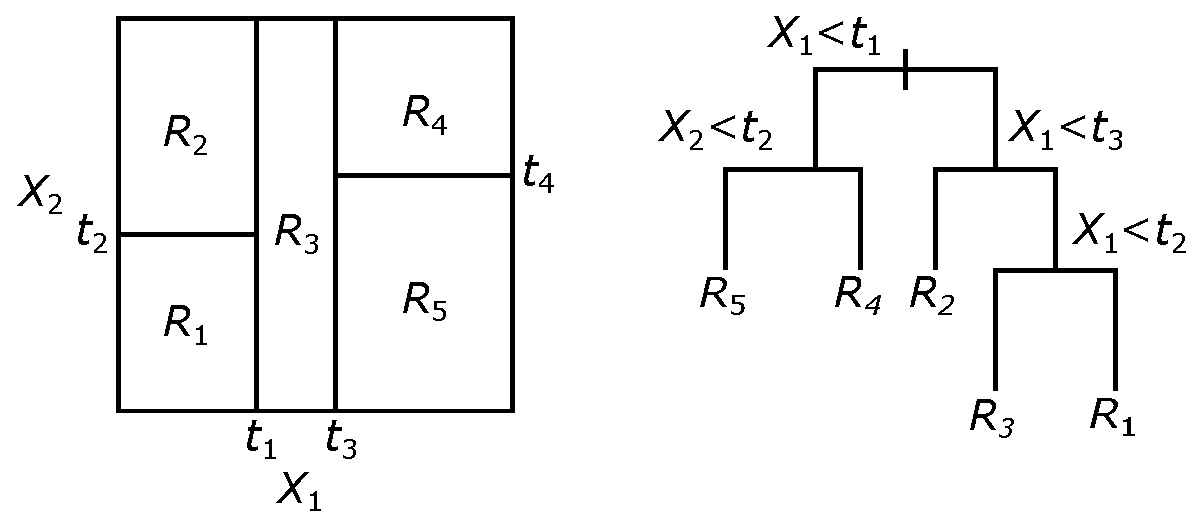
\includegraphics[width = \textwidth]{sections/TheoryGraphs/ZeichnungDecisionTree_Rectangle.eps}
		\caption[Structure of a CART split and its resulting Decision Tree]{
		The recursively binary grown split is shown on the left. On the right, the resulting Decision Tree is depicted.}
		\label{fig:ML_Split}
	\end{figure}
	In each partition $Y$ is modeled with a function or constant $R_i$.
	The splitting points $t_1$ to $t_4$ are chosen differently for the RFR and ETR.
	In RFR, the splitting point is determined by choosing the best feature and of this feature the best split value.
	Hence, it is a two dimensional search.
	In the case of the ETR, the feature is chosen randomly.
	After that, the best split value for this feature is chosen.
	The relation between the features and the partitioned response $Y$ can be depicted in a decision tree,
	which is shown in Fig.~\ref{fig:ML_Split} on the right.
	This can also be described mathematically via Eq.~\eqref{eq:DTfunc}
	\begin{align}
		\label{eq:DTfunc}
		\hat{f}(X) = \sum_{m=1}^5 c_m I\{(X_1,X_2) \in R_m \}
	\end{align}
	Here, $\hat{f}(X)$ is the function that describes the response $Y$.
	Each region $m$ has a corresponding constant $c_m$. The function $I$ can either be $I=1$,
	if the features $X_1$ and $X_2$ are in the rectangle $R_m$, or it is $I=0$, if it is not the case.
	Originally, the ETR and RFR have another difference, which is that the ETR did not use bootstrapping.
	Bootstrapping uses the training set and makes several new training sets from this.
	The new training sets are randomly filled with the datasets of the original training set.

